\begin{frame}
  \frametitle{\textbf{Deconfinement in heavy-ion collisions}}
  \begin{columns}
    \column{0.5\textwidth}
    \begin{itemize}
    %\item Discretize spacetime to lattice and simulate quark-gluon interactions $\to$ ``lattice QCD''
    \item Lattice QCD predicts that partons break away from strong-force bonds at sufficent energy density $\to$ \textbf{deconfinement}
    \end{itemize}
    \begin{itemize}
    \item Critical temperature ($T_c$)
      \begin{itemize}
      \item $T_c$ via lattice QCD / simple confinement models ($\mu_B = 0$)
      \item $T_c$ for non-zero $\mu_B$ is challenging
      \item state-of-the-art: $\boldmath{T_c \approx 158.0 \pm 0.6 \textbf{ MeV}}$
      \end{itemize}
    \item Evidence of $T_{\text{exp}} > T_c$
      \begin{itemize} 
      \item Estimations of particle ratios
        \begin{itemize}
        \item $dn_i \sim \exp\left\{ (E_i - \mu_B) / T  \right\} d^3 p_i$
        \item $\cfrac{\bar{p}}{p} = \exp\left\{-2\mu_B / T \right\}$
        \item $\cfrac{K}{\pi} = \exp\left\{-(E_K - E_\pi)/T  \right\}$
        \end{itemize}
      
   
      
      \end{itemize}

      \item System at extreme $T$ and $P$ $\to$ deconfined phase of quarks and gluons $\to$ \textbf{Quark Gluon Plasma} (QGP)

      %\item Statistical thermodynamics in QCD $\to$ $m_{\pi} \lesssim$ 140 MeV (1965)
    %\item Lattice QCD (at $\mu_B \sim 0$) $\to$ $T_C \approx 
    %\item Lattice QCD predicts a deconfined phase of quarks and gluons known as the \textbf{Quark Gluon Plasma} at extreme temperatures and pressures
    %\item At $\mu_B \sim 0$, the critical temperature for this phase-change is $\boldmath{T_c \approx 158.0 \pm 0.6 \textbf{ MeV} \approx 1.8 \cdot 10^{12} \textbf{ K}}$
    \end{itemize}
    \column{0.5\textwidth}
    \centering 
    \begin{tikzpicture}
      \node{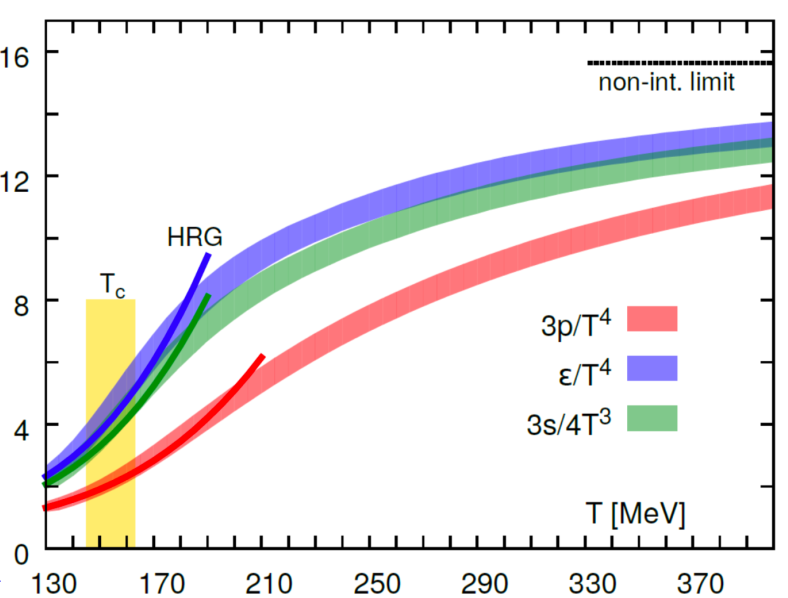
\includegraphics[width=0.8\textwidth]{qcd-phase-change-alt.png}};
      \node[font=\tiny,align=left] at (1.2,2.0) {\textbf{Lattice QCD phase change}};
      \node[font=\scriptsize,align=left] at (-1,1.5) {$\boldmath{\mu_B = 0}$};
      \node[font=\scriptsize,align=left,rotate=90] at (-2.6,0.7) {Degrees of freedom};
      %\node[font=\tiny,align=left] at (1.2,1.6) {\href{https://doi.org/10.1016/j.physletb.2019.07.014}{https://doi.org/10.1016/j.physletb.2019.07.014}};
    \end{tikzpicture}

    \

    \begin{tikzpicture}
      \node{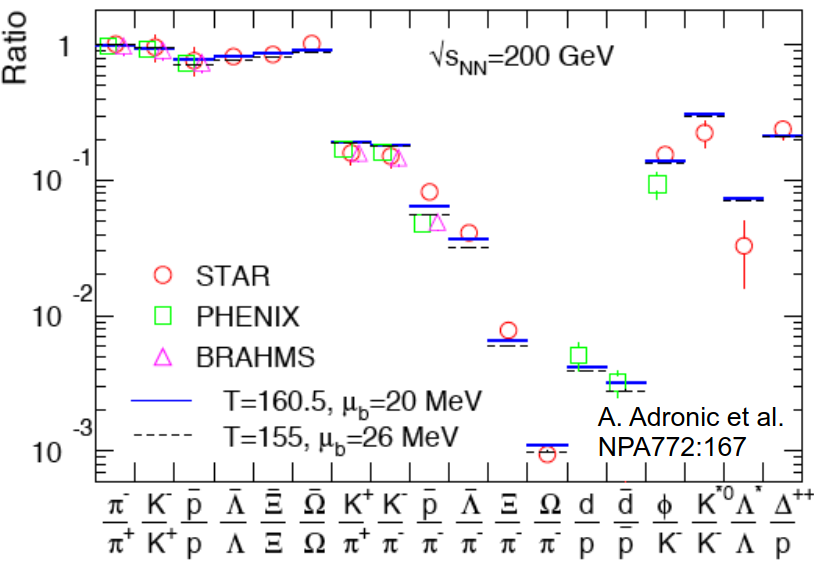
\includegraphics[width=0.8\textwidth]{particle-ratios.png}};
      \node[font=\tiny,align=left] at (1.2,1.85) {\textbf{Particle ratios at RHIC}};
    \end{tikzpicture}
%    \begin{tikzpicture}
%      \node{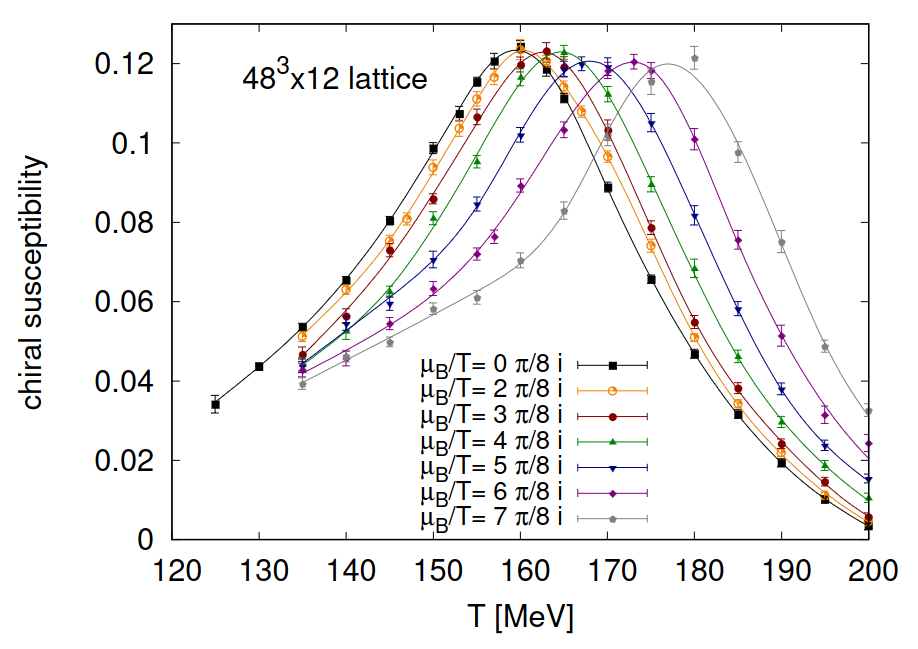
\includegraphics[width=0.9\textwidth]{chiral-susceptibility.png}};
%      \node[font=\tiny,align=left] at (1.2,1.6) {\href{https://arxiv.org/abs/2002.02821}{arXiv:2002.02821}};
%    \end{tikzpicture}
  \end{columns}
\end{frame}
